\documentclass{article}
\usepackage[utf8]{inputenc}
\usepackage[a4paper, total={6in, 9in}]{geometry}
 
\usepackage[smartEllipses]{markdown}
\usepackage{enumitem}
\usepackage{hyperref}
\usepackage{caption}
\usepackage{minted}
\usepackage{amsmath}



\title{
Elaborato di Matematica e Fisica:\\
Di forni a microonde, elettromagnetismo e crisi 
\vspace{1mm} %5mm vertical space

}
\author{Francesco Genovese, 5C Liceo Scientifico D. Bramante}
\date{A.S. 2020/2021}


\begin{document}

\maketitle
\vspace*{-0.2in}
\begin{abstract}
%da rifare
Si discutono  l'elettromagnetismo, il comportamento ondulatorio o quantizzato della luce e la crisi della fisica classica analizzando le componenti ed il funzionamento del forno a microonde. Si osserva in particolare il processo ed il moto che porta alla produzione di microonde nel magnetron e si avvalorano le spiegazioni con le leggi di Maxwell. Si introduce il concetto di integrale,  si studiano due funzioni relative al comportamento della luce e si conclude sottolineando nuovamente lo spessore rivoluzionario dell'elettromagnetismo per la nascita della fisica quantistica. 
\end{abstract}

\tableofcontents

\paragraph{Docente tutor:} Massimiliano Luppi
\paragraph{Digest allegati esterni}
Si allega il digest md5 del codice inserito all'interno dell'IDE \href{https://editor.p5js.org/}{\underline{P5JS}} al fine di controprovarne alterazioni postume alla consegna dell'elaborato. Il digest è realizzato con \href{https://emn178.github.io/online-tools/md5.html}{\underline{questo tool online}}.
\begin{enumerate}[noitemsep]
\item Animazione n. 1: \textit{0fb2c9c97967c3d09ba0a8feab4302b5}
\item Animazione n. 2: \textit{2657875efc537e8ef4a828deac7ee3bc}

\end{enumerate}
\newpage

\section{Dalla fisica di Newton alle Microonde: una rivoluzione}
\subsection{Una provocazione}
\begin{quote}
Uno spettro si aggira per l’Europa – lo spettro dell’elettromagnetismo. Tutte le scienze della vecchia Europa, la fisica e la chimica, Galileo e Newton, deterministi e causalisti, meccanicisti e Laplaciani, Michelson e Morley,  si sono uniti in crociata e danno la caccia a questo spettro
\footnote{Citazione al manifesto del partito comunista: 
\begin{quote}
Uno spettro si aggira per l’Europa – lo spettro del comunismo. Tutte le potenze della vecchia Europa, il papa e lo
zar, Metternich e Guizot, i radicali francesi e i poliziotti
tedeschi, si sono unite in una crociata e in una caccia spietata contro questo spettro. 
\end{quote}
}
\end{quote}

%sistemare%


Quello presentato, in realtà, è un fantasma fittizio: la crociata sopra descritta non è che figurativa, molti dei “cacciatori” citati, già scomparsi o non ancora nati all’epoca, sarebbero stati più che contenti di essere smentiti. Le scoperte che riguardano la natura delle sostanze ferromagnetiche da parte di Faraday ed Oersted sono infatti ben accolte dalla comunità scientifica. Queste entrano però presto in contrapposizione dialettica, in antitesi, con la fisica dei secoli prima: le equazioni di Maxwell, che descrivono il comportamento della luce, scopertasi onda elettromagnetica, sono incompatibili con la dinamica e la meccanica classica. Vi sono delle incongruenze fra i due modelli che vanno a sommarsi  alle domande lasciate senza risposta dalla concezione della forza di gravità di Newton come attrazione invisibile e indecifrabile. Dalle trasformazioni di Galileo, che non contemplano l'invarianza della luce, alla definizioni di energia totale, cinetica e della quantità di moto, qualcosa non quadra.
\\

In questo scenario, si potrebbe dire provocatoriamente che, in modo analogo al proletariato, l’elettromagnetismo ricopra una carica eversiva e rivoluzionaria all’interno dello studio della fisica. Solleva quesiti nuovi, mettendo in luce le criticità necessarie di una conoscenza induttiva e modellistica del mondo naturale, anche se, come spesso accade, finisce per lasciare più interrogativi aperti che chiusi. Questo è però il bello della scienza, dopotutto.
\\

Le resistenze incontrate e confutate, a partire dalla concezione dell’etere luminifero e dunque dall’esperimento di Michelson e Morley attraverso l'interferometro, hanno fatto sì che lo studio della fisica, un processo appunto dialettico, giungesse alla relatività ristretta, sintesi della dinamica classica entrata in attrito con il principio di invarianza della luce, poi alla relatività generale, soluzione al conflitto tra relatività ristretta e meccanica classica ed infine, più tardi, alla concezione, sempre per sintesi Hegeliana, della meccanica quantistica che dava finalmente spiegazione alla doppia natura del comportamento della luce.
\\

Lo studio delle onde elettromagnetiche e dunque della luce ci ha permesso di sostituire al mondo freddo, piatto e meccanico concepito da Newton e Laplace ‒ fatto di  minuscoli sassolini freddi che vagavano eterni lungo traiettorie precise di uno spazio geometrico ‒ un mondo più elegante, formato da moti più semplici, rettilinei  ed uniformi, ma che all’interno dello spazio tempo, incurvato da masse, non più assolute, si configurano nei moti ellittici, accelerati, e combinati a cui assistiamo per mezzo dei nostri telescopi. 
\\ %logica del concreto

Si potrebbe azzardare, almeno per quanto riguarda lo studio della fisica, che l’elettromagnetismo metta finalmente in crisi la concezione provvidenzialistica del mondo,  governato da principi e leggi immutabili, approdando ad un mondo nuovo, sconosciuto e indeterminato, che non contempli motori immobili e arcani rapporti causali a noi oscuri. 

\newpage
\subsection{Di Maxwell, Prometeo e dei Forni a Micronde}
Le equazioni di Maxwell cambiano radicalmente il volto della fisica, non vi sono più particelle che si influenzano attraverso misteriose interazioni a distanza, ma particelle che interagiscono per mezzo di campi, del campo elettromagnetico. La rivoluzionarietà del concetto di campo non si limita alla fisica teorica. Le applicazioni reali di questi leggi, infatti, sono vastissime. 
\\

Ad esempio, banalmente, grazie ad esse oggi siamo in grado di riscaldare e volendo cucinare del cibo attraverso l’uso di un forno a microonde, dispositivo che ci apprestiamo ad analizzare. In un certo senso, Maxwell e Faraday sono i Prometeo dei tempi moderni.





\section{Il forno a microonde}
\subsection{Le componenti del microonde}


Un forno a microonde è un dispositivo che sfrutta onde elettromagnetiche a frequenza $f$ relativamente bassa per riscaldare e cuocere degli alimenti. Si tratta di onde che hanno una lunghezza d’onda $\lambda$ maggiore rispetto allo spettro delle onde elettromagnetiche visibili. La lunghezza d’onda è compresa tra quelle delle onde radio e delle radiazioni infrarosse, ed è in genere tra \textit{1 m}e \textit{1 mm.}

Ricordiamo che $c = \lambda f $

\begin{figure}[h]
\centering
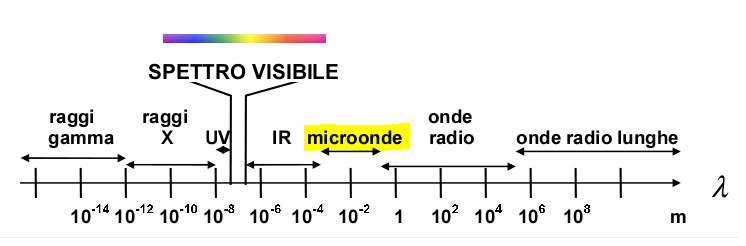
\includegraphics[scale=0.6]{1.PNG}
\label{fig: cubed graph}
\end{figure}





Un forno a microonde si compone delle seguenti parti: 
\begin{itemize}[noitemsep]
\item Un \textbf{trasformatore}: che innalzi il valore della tensione della corrente. 
\item Un \textbf{raddrizzatore} che assicuri un flusso di \textit{corrente elettrica continua} e non alternata al magnetron.
\item  Un\textbf{ magnetron}, all'interno del quale vengono generate le onde elettromagnetiche.
\item Un \textbf{circuito di controllo} per il magnetron funzionale alla gestione elettrica del magnetron e dunque alla modulazione delle microonde. La modulazione avviene per mezzo di un microprocessore. 
\item Un \textbf{vacuum tube}, un tubo d'aspirazione che mantiene il vuoto all'interno del magnetron.
\item Una \textbf{ventola} che tenga freddo il magnetron.
\item Una \textbf{guida d’onda} che indirizza le onde elettromagnetiche dal magnetron alla camera di cottura.
\item Una camera o \textbf{cavità di cottura}  contente in genere un piatto rotante.
\item Una\textbf{ rete in metallo} applicata allo sportello che blocchi le radiazioni che tentano di sfuggire alla cavità di cottura.

\begin{figure}[h]
\centering
\frame{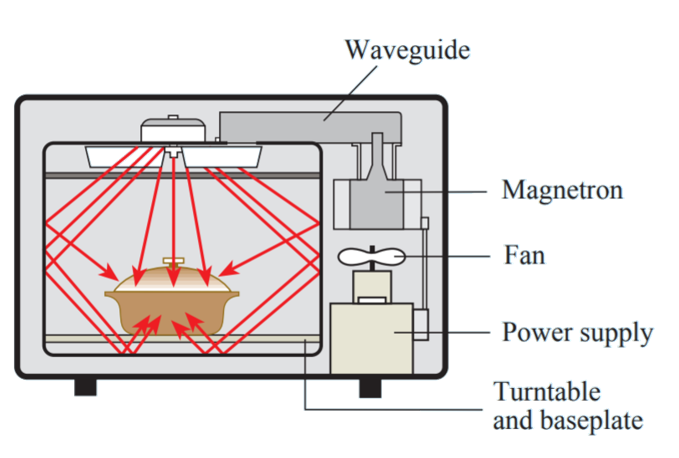
\includegraphics[scale=0.50]{3.png}}
\label{fig: cubed graph}
\end{figure}
\end{itemize}
\subsection{Trasformatore e Raddrizzatore  }
\paragraph{Il trasformatore.}
Affinché il magnetron riesca a generare delle onde elettromagnetiche, c'è bisogno che questo sia alimentato da una tensione in corrente continua di diverse migliaia di Volt.
A tal proposito, per innalzare il valore della tensione della corrente proveniente dalla rete elettrica ($fem_{eff,0} = 400V$) si utilizza il dispositivo del trasformatore che sfrutta il fenomeno dell'induzione elettromagnetica per innalzare ed abbassare la tensione o la corrente a seconda delle sue caratteristiche costruttive. Il forno microonde utilizza un trasformatore di tensione.
\\

Un trasformatore è composto da due bobine, due solenoidi, di resistenza trascurabile avvolti attorno ad un nucleo di ferro. Possiamo distinguere due circuiti: uno primario ed uno secondario.
Nel circuito primario, la corrente alternata in entrata proveniente dalla rete elettrica genera un campo magnetico variabile. Come sappiamo infatti dall'esperienza di Oerstead, un filo percorso da corrente genera un campo magnetico. Precisamente, nel caso del solenoide si tratta di un campo magnetico dal modulo $ B_1 = \mu_0 \frac{N_1}{l}i $ . Il campo magnetico variabile viene aumentato di intensità ed indirizzato dal nucleo di ferro che lega i due solenoidi. Il ferro, sostanza paramagnetica dal forte momento magnetico, agisce in modo tale che le perdite di potenza non siano troppo significative: 
\begin{center}
$\Delta P \approx 0  \to  i_{eff,2}f_{eff,2}- i_{eff,1}f_{eff,1} \approx  0$ 
\end{center}

All'interno del circuito secondario, la variazione di flusso del campo magnetico, in accordo con la legge di Faraday-Neumann genera una corrente indotta, poiché il modulo del campo magnetico che investe la superficie del solenoide del circuito secondario varia poiché generato da una corrente alternata. Dalla seconda legge di Maxwell e dalla prima legge di Ohm: 
\begin{center}
 $i_{2 indotta} = \frac{f_{eff}}{R} = -\frac{\Delta\Phi_{1,2}(B)}{\Delta t} \frac{1}{R} = -\frac{\Delta B \ \Delta S \ cos(\widehat{BS})}{\Delta t}\frac{1}{R}$ 
\end{center}
Valgono dunque: 
\begin{center}
$f_{em,1} = -N \frac{d\Phi}{dt} \ $ e \  $f_{em,2} = -N \frac{d\Phi}{dt}$   
\end{center}
Se non si dissipa potenza allora 
\begin{center}
$\Delta P \approx 0  \to \frac{f_{em,2}}{f_{em,1} } = \frac{N_2 }{N_1}$
\end{center}
Affinchè la tensione sia innalzata, il rapporto di 
trasformazione $\frac{N_2 }{N_1}$ dovrà essere $>1$ e dunque il numero di spire $N_2 > N_1$
\paragraph{Il raddrizzatore.}
Una volta trasformata la tensione, un piccolo dispositivo, il raddrizzatore, si occupa di trasformare la corrente alternata in  nel suo valore efficace, il corrispondente continuo.

Dato che in un circuito Ohmico di Resistenza R attraversato da corrente alternata la potenza dissipata per effetto Joule corrisponde a $ p (t) = R\ i_0^2\ sen(\omega t)$ avremo allora l'erogazione di una potenza media pari a $\overline{P} = \frac{1}{2} Ri_0^2$ 
\begin{figure}[h]
\centering
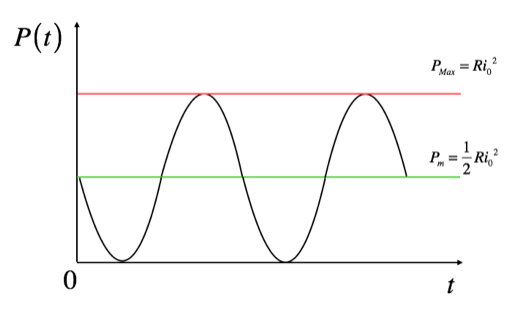
\includegraphics[scale=0.30]{4.png}
\label{fig: cubed graph}
\end{figure}

La potenza $\overline{P}$ è prodotta allo stesso modo da una corrente continua di Intensità efficace $i_{eff}= \frac{i_0}{\sqrt{2}}$. Il raddrizzatore si occupa appunto del raddrizzamento del segnale alternato in uno mono-direzionale, senza perdite significative di potenza $\Delta P \approx 0  \to P_{eff} -\overline{P} \approx 0$ .
Per la legge di Ohm avremo dunque:
\begin{center}
$V_{eff}= \frac{V_0}{\sqrt{2}} =  \frac{i_{eff}}{R}= \frac{i_0}{\sqrt{2}\ R} $
\end{center}
\newpage

% Inserire il condensatore ?
\subsection{Magnetron: tra condensatore ed induttore}
La corrente continua arriva infine al magnetron, un dispositivo cilindrico, fondamentale per il funzionamento di un forno a microonde, che si occupa della generazione delle onde elettromagnetiche che riscalderanno gli alimenti.
\paragraph{L'effetto termoionico} Il raddrizzamento si rivela un passaggio fondamentale per il funzionamento del magnetron: la corrente continua percorre un solenoide che funge da antenna. Questo, per effetto Joule, si riscalda. Con l'aumento della temperatura abbiamo un aumento dell'energia cinetica media degli elettroni, liberi all'interno del metallo. Tra l'esterno e l'interno vi è una differenza di potenziale che viene colmata dall'energia termica e dunque cinetica degli elettroni. 
\begin{center}
$V_{estrazione} = \frac{W_{estrazione}}{e}$ con $e$ carica elementare
\end{center}
Una volta superata la soglia del lavoro di estrazione, l'elettrone viene liberato dal metallo. Il metallo rimane  ionizzato poiché privo di elettroni: L'elettrone sfugge all'antenna per effetto termoionico.
\paragraph{Il magnetron come condensatore}
Gli elettroni liberati dall'antenna entrano nella cavità del magnetron, si formano un anodo ed un catodo per la differenza di potenziale: vi sono molti elettroni attorno all'antenna. Si crea dunque un campo elettrico dal catodo (esterno, positivo) all'anodo (interno, negativo). 
 \[ E =  \frac{\Delta V}{S}\]
 \vspace*{-0.25in}
\begin{figure}[h]
\centering
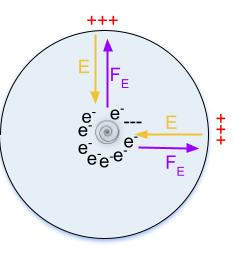
\includegraphics[scale=0.36
]{6.png}
\label{fig: cubed graph}
\end{figure}\\
Ecco che allora il magnetron si comporta come un condensatore: sebbene non sia piano, possiamo trovare una armatura positiva, la superficie esterna del magnetron, ed una negativa, l'antenna. Esse sono isolate dallo spazio vuoto creato dal tubo di aspirazione. Troviamo un campo elettrico  uscente rispetto alla piastra positiva, poiché le linee di campo elettrico sono in generale entranti rispetto a cariche negative. Le cariche, immerse in un campo magnetico, subiscono una forza pari a:  
\begin{center}
$ F= q E = -e E$ con $e$ carica elementare    
\end{center}

Gli elettroni, secondo il loro moto spontaneo, salgono la curva del potenziale, passando da un punto a potenziale maggiore, vicini all'antenna, a punti a potenziale minore cioè verso l'armatura positiva. Se chiamiamo A il punto dell'antenna e B un punto dell'armatura positiva possiamo dimostrare come il moto sia  spontaneo:

\begin{center}
Se $ W_{A\to B} > 0 \to$ moto spontaneo  \\ 
$W_{A\to B} = F\Delta S =  q \ E \ \Delta z  = q \ \Delta V =  -e (V_{B} - V_{A})$  \\
 $ W_{A\to B} > 0$ poiché $V_{B} < V_{A}$  e $-e<0$  \\
\end{center}
\vspace*{-0.2in}
\begin{figure}[h]
\centering
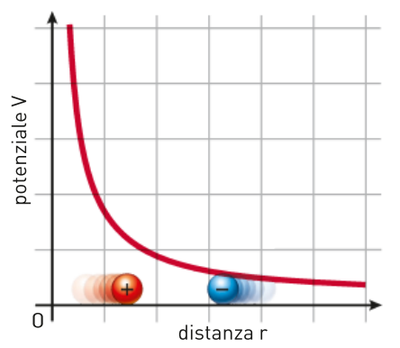
\includegraphics[scale=0.23]{7.png}
\label{fig: cubed graph}
\end{figure}

\newpage
\paragraph{Il magnetron come induttore}
Abbiamo visto che il magnetron si comporta come un condensatore, genera un campo elettrico fra anodo e catodo che accelera il moto delle cariche. Questo contribuisce a generare onde elettromagnetiche poiché, come vedremo, l'accelerazione degli elettroni genera una variazione di flusso del campo elettrico all'interno della cavità di induzione. Tuttavia, le cariche, sottoposte solo alla forza di Coulomb, rimangono troppo poco tempo nella cavità del magnetron, fra i due elettrodi, per produrre un'oscillazione e dunque un'onda che sia funzionale alla cottura. \\ 

Affinché la variazione di flusso del campo elettrico sia maggiore, si inserisce il magnetron fra due facce con polarità opposta di due magneti, posti sopra e sotto il magnetron. Creiamo così un magnete permanente, le linee di campo magnetico uscenti dalla faccia negativa del magnete inferiore entrano nella faccia positiva del magnete superiore. Il magnetron è quindi percorso da un campo magnetico uniforme. \\

Gli elettroni, che viaggiano all'interno del campo magnetico, subiscono, oltre alla forza elettrica dovuta alla differenza di potenziale, la forza di Lorentz. 
Questa forza, $\overrightarrow{ F_L} = q \ \overrightarrow{v}  \times \overrightarrow{B}$,  ha lavoro pari a zero poiché l'angolo $\widehat{F_{L} \Delta S} = \widehat{F_{L} V_{e^-} $  è sempre di $90$°. 
Per il teorema dell'energia cinetica il lavoro è uguale alla variazione dell'energia cinetica: 
\begin{center}
    $ W = F \times \Delta S = F_{L} \cdot V \cdot t \cdot cos(\widehat{F_L \ V}) =  \Delta K = \frac{1}{2}m_{e} (V_f^2 - V_i^2) $\\ dunque se $ W = 0 \to \Delta k =0 \wedge V_f = V_i$
\end{center}
Poiché la velocità non varia, la Forza di Lorentz funge da forza centripeta che fa percorrere all'elettrone un moto circolare uniforme.
\\
Questo moto, che si compone allo spostamento delle cariche dovuto al campo elettrico, su cui ora agiscono la forza di Coulomb e di Lorentz, si configura nella curva rossa nel grafico sotto riportato, che va a modificare la traiettoria rettilinea dall'anodo al catodo di cui prima. Otteniamo così una variazione di flusso del campo elettrico maggiore, dovuta allo spostamento curvilineo delle cariche

\begin{figure}[h]
\centering
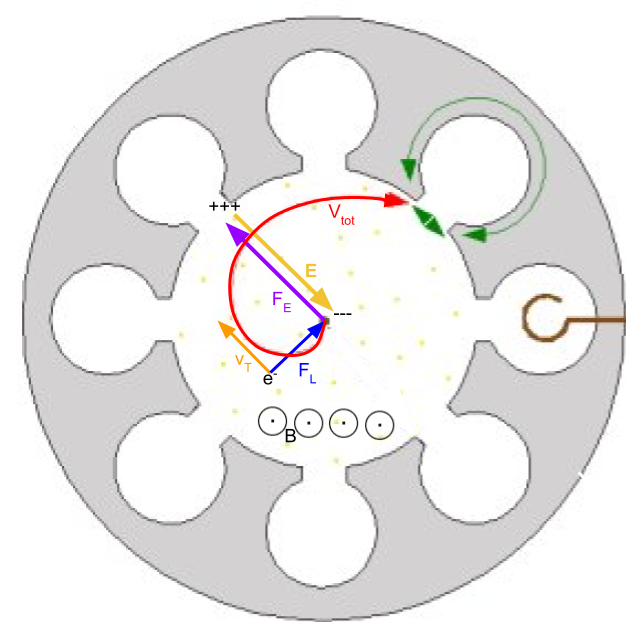
\includegraphics[scale=0.25]{5.png}
\label{fig: cubed graph}
\end{figure}
L'efficienza viene ulteriormente migliorata quando vengono introdotte delle cavità di risonanza ulteriori alla camera induttiva o spazio di interazione (la circonferenza principale). Il moto composito degli elettroni va a spostare gli elettroni liberi presenti all'interno del catodo, creando una corrente indotta, che ha la direzione della curva verde nel grafico riportato sopra. 
\\

Questa corrente, indotta, oscilla tra i due estremi di ogni camera di risonanza poiché gli elettroni al suo interno sono indotti a spostarsi dal moto degli elettroni che si muovono all'interno dello spazio di interazione per la forza di Coulomb e di Lorentz. Allo stesso modo, gli elettroni nello spazio di interazione emessi dall'anodo sono deviati anche essi verso le sezioni positive delle camere di risonanza, verso punti a potenziale maggiore, dove la carica è positiva. 
\\

Poiché la superficie del catodo si comporta come una serie di condensatori rotanti, positiva e negativa ad intervalli regolari in alternanza fra loro, il movimento degli elettroni nello spazio di interazione genera una figura particolare, una sorta di stella rotante dai bracci spiraliformi, che provoca un cambiamento del flusso del campo magnetico all'interno dello spazio di interazione. È proprio questo genere di figura che determina il moto degli elettroni necessario per produrre  onde elettromagnetiche — e duque oscillazioni di elettroni — dalla lunghezza d'onda delle microonde.  
\begin{figure}[h]
    \centering
    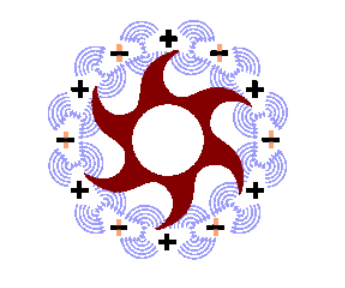
\includegraphics[scale=0.60]{8.PNG} 
    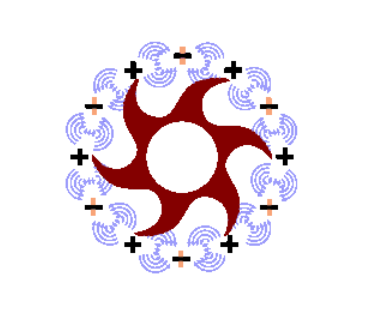
\includegraphics[scale=0.60]{9.PNG}
    \caption*{\href{https://www.radartutorial.eu/08.transmitters/pic/mag06.gif}{\textit{\underline{Cliccare qui per l'animazione}}}}
    \label{}
\end{figure}
\subsection{Animando il magnetron}
Seguiamo il moto dei singoli elettroni con una animazione realizzata in p5JS, una libreria del linguaggio di scripting web Javascript, ogni elettrone è un oggetto indipendente, un'istanza singola della classe elettrone con i propri metodi che lo fanno muovere: 
Riportiamo i passaggi più importanti
  {\scriptsize \begin{minted}{javascript}
let electrons = [];
class electron{
	//metodo costruttore
	constructor(x,y,a,r){
		this.x= x;        
		this.y = y;     
		this.a = a; //angolo
		this.r = r;  //distanza dal centro
		this.rSpeed= 10;
		this.tSpeed= 35.88;
	}
	//metodo che muove gli elettroni
	move(){
		//gli elettroni si muovono di moto rettilineo
		this.r = this.r + this.rSpeed;
		//composto ad un moto circolare uniforme
        this.a = this.a + this.tSpeed;
		this.x = cx+this.r*cos(+this.a); 
		this.y = cy+this.r*sin(-this.a);
	}
	//metodo che visualizza gli elettroni sul canvas
	show(){ ellipse(this.x,this.y,5);} 
}
//Setup
function setup() {
	for(var i=0;i<10;i++){  // seguiamo il moto di 10 elettroni
		e= new electron(windowWidth/2,windowHeight/2,360/10*i,45);
		electrons.push(e);
	}
}

//loop per disegnare
function draw() {
	cx = windowWidth/2; cy = windowHeight/2;
	ellipse(cx,cy,100); ellipse(cx,cy,50);   //disegno il solenoide
	for(let electron of electrons){
		if(dist(cx, cy, electron.x, electron.y)<200){
			electron.move();
			electron.show();
		}
	}
}
\end{minted} } 
\href{https://editor.p5js.org/freihm15@gmail.com/sketches/Ibo6ae2T1}{\textit{Apri l'editor cliccando qui}}
  
\section{Il magnetron e le equazioni di Maxwell}
}
\paragraph {Faraday ed i campi} L'analisi del funzionamento del magnetron svolta, ci è resa possibile dall'intuizione del concetto di campo da parte del Londinese Micheal Faraday, che condusse una vita veramente umile, nella povertà, senza mai ricevere alcuna istruzione formale, ma che si rivelò poi il più grande sperimentatore e visionario della fisica moderna. Da buon Newtoniano, egli cerca inizialmente di capire quali proprietà avessero gli oggetti carichi e magnetici. Ha però poi un'intuizione rivoluzionaria, quella di un'entità diffusa ovunque nello spazio, il campo elettromagnetico, che è modificato da corpi carichi e magnetici che quindi spingono o tirano gli altri corpi. È un campo che per analogia possiamo paragonare a quello che concepirà Einstein con la relatività generale, proprio pensando a quello elettromagnetico: quello spazio-temporale.

\begin{figure}[h]
    \centering
    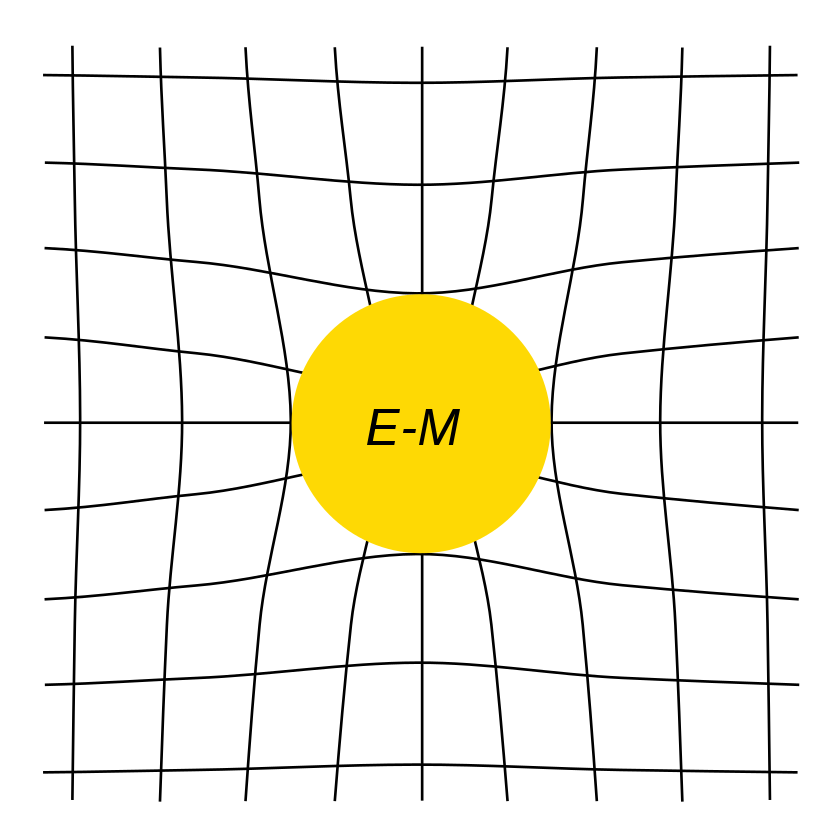
\includegraphics[scale=0.20]{10.png} 
    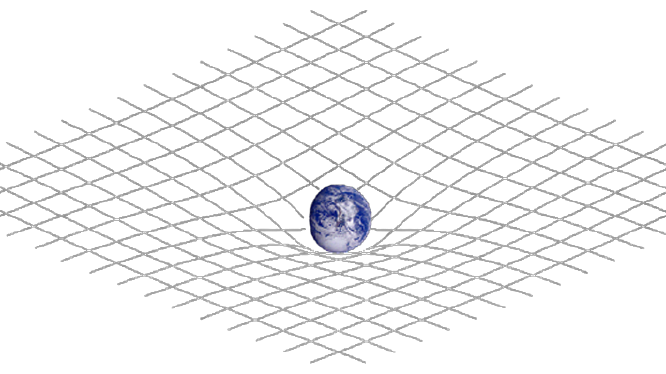
\includegraphics[scale=0.20]{11.png} 
    \label{example}
\end{figure}
\paragraph{Maxwell ed i campi}
Tornando all'elettromagnetismo, James Clerk Maxwell, di origine aristocratica, che invece un'educazione formale la aveva eccome —giusto per dire che il conflitto di classe lo troviamo anche nella fisica — capisce quanto la fisica dei campi sia rivoluzionaria anche dal punto di vista matematico. Sviluppa così un set di 4 equazioni che spiegano il comportamento del campo elettrico e magnetico, che scopriamo dipendenti ed imprescindibili l'uno dall'altro.
Queste equazioni avvalorano quanto abbiamo visto fin'ora sul comportamento del magnetron. Riepiloghiamolo brevemente:

\subsection{La prima equazione di Maxwell}
\begin{center}
$\Phi_\Omega (\overrightarrow{E})  = \frac {Q_{Tot}}{\varepsilon_0} $
\end{center}
Vediamo che il flusso del campo elettrico $\overrightarrow{E}$ attraverso una superficie chiusa Omega dipende dalla Quantità di carica sulla la costante dielettrica del vuoto. Le cariche, dunque, come osserviamo all'emissione di cariche da parte del solenoide all'interno dello spazio di interazione del magnetron, sono sorgenti di un campo elettrico.

\subsection{La seconda equazione di Maxwell}
\begin{center}
$\Gamma_{\mathcal{L}} (\overrightarrow{E}) = - \frac{\Delta\Phi_{S}(\overrightarrow{B})}{\Delta t} = f_{em}$
\end{center}
\\ Vediamo che la circuitazione del campo Elettrico $\overrightarrow{E}$ una linea chiusa $\mathcal{L}$ é uguale alla variazione del flusso del campo magnetico cambiata di segno attraverso una superficie S delimitata dalla linea chiusa e orientata $\mathcal{L}$ sul tempo.
\\ Vale a dire che, come vediamo nel perimetro interno dell'anodo, la variazione del campo magnetico, generato all'interno dello spazio di interazione dal campo elettrico variabile, produce corrente indotta e quindi un campo elettrico fra gli estremi opposti nella camera di induzione. 
Se invertiamo la formula vediamo che la corrente indotta genera una variazione della quantità del flusso del campo magnetico, nel nostro caso producendo la figura rotante, a stella, che abbiamo visto.
\begin{center}
$\Delta\Phi_{S}(\overrightarrow{B}) = -  \Gamma_{\mathcal{L}} (\overrightarrow{E}) \Delta t = f_{em}\Delta t$
\end{center}
\subsection{La terza equazione di Maxwell}
\begin{center}
$\Phi_\Omega (B) = 0 $
\end{center}
\\ Come enuncia il teorema di Gauss, il flusso totale che attraversa una superficie chiusa $\Omega$ è zero. Se prendiamo il nostro magnetron cilindrico, sulla superficie laterale avranno $\Phi_\Omega (B) = B \ 2\pi r h  \cos(90°)$ = 0 e il flusso del campo magnetico attraverso la  superficie sopra e sotto, eccetto quello incanalato nella guida d'onda, è pari a 0 poiché possiede in entrambi i poli lo stesso modulo ma con verso opposto. Scopriamo curiosamente che il flusso di campo magnetico che farebbe interferenza con altre componenti del microonde è pari a 0.
\subsection{La quarta equazione di Maxwell}
\begin{center}
$\Gamma_{\mathcal{L}}(\overrightarrow{B}) = \mu_0 \ [i_{tot}+ \varepsilon_0 \frac{\Delta \Phi_{S}(\overrightarrow{E})}{\Delta t}]$
\end{center} 
La circuitazione del campo elettrico è uguale alla costante di permeabilità magnetica per la corrente totale più la corrente di spostamento. Le  sorgenti del campo magnetico sono, come si assiste nel caso del nostro magnetron, le correnti elettriche (nel nostro caso il solenoide e le correnti nella camera di risonanza) ed i campi elettrici variabili, come assistiamo all'interno dello spazio di interazione del magnetron. 

\subsection{Delle conclusioni }
Come prima Faraday – fisicamente –  e poi Maxwell – matematicamente– capiscono, i fenomeni che riguardano campo magnetico e campo elettrico sono due facce della stessa medaglia. 
Un elettrone che oscilli due punti produce
\begin{itemize}[noitemsep]
\item Un campo elettrico variabile perché la carica cambia continuamente posizione 
\item Un campo magnetico variabile poiché la carica elettrica che oscilla equivale ad una corrente elettrica alternata.
\end{itemize}
Per effetto delle oscillazioni di una carica si genera un campo elettrico variabile, il campo elettrico variabile genera un campo magnetico variabile in un altro punto, il campo magnetico così prodotto dà origine ad un altro campo  elettrico indotto. Si propaga così un'onda elettromagnetica, una perturbazione del campo elettromagnetico che porta con sé energia e quantità di moto 
Un'Onda elettromagnetica continua a propagarsi anche quando la carica che l'ha generata smette di muoversi. \\
\begin{center}
$
\left\{\begin{array}{@{}l@{}}
   		c = \frac{1}{\sqrt{\mu_0 \varepsilon_0}}, \\
      E = cB , \\
      f = c \lambda
  \end{array}\right.\,.
$
\end{center}

 \begin{figure}[h]
\centering
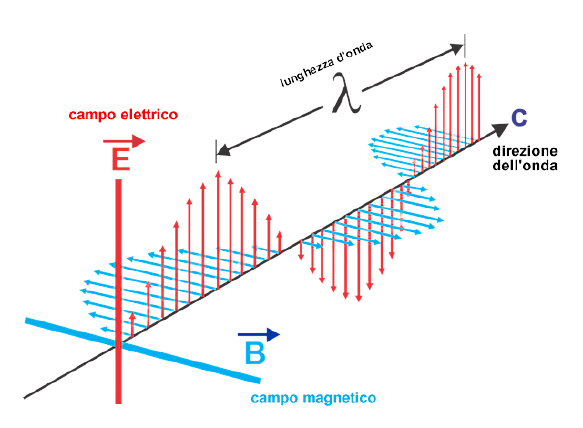
\includegraphics[scale=0.28]{12.png}
\label{fig: cubed graph}
\end{figure}

\newpage
\section{La cottura ed il riscaldamento a microonde }
\subsection{Lo spin delle molecole d'acqua} 
Una volta generate, le onde elettromagnetiche vengono condotte nella cavità di cottura per mezzo della guida d'onda, un tubo dalla sezione rettangolare. 
Le onde elettromagnetiche cominciano qui la cottura o il riscaldamento degli alimenti attraverso la rotazione, lo spinning, di molecole polari. Queste, sottoposte ad un campo elettrico variabile, cambiano continuamente orientamento poiché i dipoli magnetici della molecola sono attratti dal potenziale elettrico opposto.\\ 

Nel caso specifico dei forni a microonde commercialmente usati, la molecola target delle oscillazioni delle microonde con una specifica lunghezza d'onda generata dal magnetron è l'acqua. 
L'acqua, inserita nel campo elettrico, acquisisce velocità aumentando la propria temperatura.\\

In accordo con il secondo principio della termodinamica – secondo il quale non è possibile costruire una macchina il cui unico scopo sia quello di trasportare calore da un corpo più caldo ad uno più freddo – ma più in generale le leggi probabilistiche di Boltzmann – secondo le quali è semplicemente più probabile che una molecola a temperatura (e dunque velocità) elevata compia un urto efficace con un'altra molecola cedendole calore– l'acqua cede energia alle altre molecole sotto forma di calore riscaldando tutto il contenuto del microonde.
\vspace*{-0.15in}
 \begin{figure}[h]
\centering
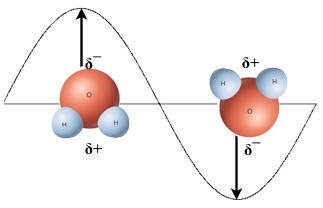
\includegraphics[scale=0.25]{13.png}
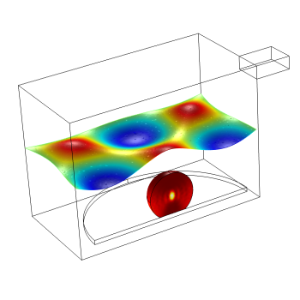
\includegraphics[scale=0.21]{19.png}

\label{fig: cubed graph}
\end{figure}
\vspace*{-0.3in}
\paragraph{Differenze con i forni a conduzione} La differenza dunque con i forni a convezione, che prima riscaldano l'aria, poi la superficie degli alimenti e solo poi il loro interno, è il numero totale di urti efficaci richiesti. I forni a microonde si rivelano infatti estremamente rapidi rispetto ai loro simili a convezione anche per la loro capacità di cuocere dall'interno, accelerando le molecole d'acqua per mezzo delle onde elettromagnetiche. 

\begin{figure}[h]
\centering
\frame{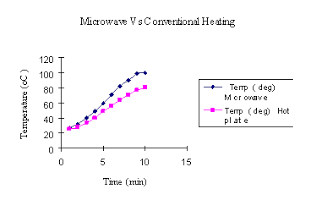
\includegraphics[scale=0.63]{14.png}}
\label{fig: cubed graph}
\end{figure}
\vspace*{-0.3in}
\subsection{Il piatto rotante}
\paragraph{Le microonde: onde stazionarie} Le onde elettromagnetiche nella camera di cottura ricordano delle onde stazionarie, aventi dei nodi fissi, poiché il flusso dei campi elettrico e magnetico, e quindi il loro profilo spaziale, è influenzato dalla sezione regolare della guida d'onda da cui escono e dalla dimensione fissa della cavità che percorrono.\\
Poiché la lunghezza d'onda delle microonde e le dimensioni lineari della camera di cottura sono all'incirca le stesse, l'irraggiamento non è identico in tutti i punti del microonde: esso sarà inferiore soprattutto nei punti di nodo, motivo per cui si inserisce un piatto rotante che promuova una cottura uniforme del cibo. È consigliabile quindi lasciare gli alimenti sul bordo del piatto del microonde piuttosto che in mezzo.     
 \begin{figure}[h]
\centering
\frame{
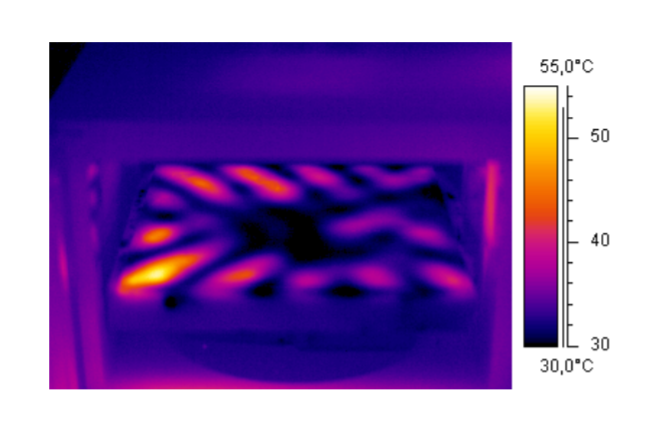
\includegraphics[scale=0.280]{15.png}}
\label{fig: cubed graph}
\end{figure}



\section{Il comportamento delle onde elettromagnetiche e la quantizzazione}
Le onde elettromagnetiche non sfuggono alla cavità di cottura poiché è realizzata come una gabbia di Faraday. La rete ferromagnetica sullo sportello assorbe tutte le onde elettromagnetiche camera.
\subsection{Cosa succede dal punto di vista Energetico all'interno della camera di cottura? 
}
\paragraph{Dubbi sull'elettromagnetismo classico}
Sebbene il modello ondulatorio delle onde elettromagnetiche spieghi come accada il riscaldamento attraverso le microonde, non è chiaro come il primo principio della termodinamica, un'estensione del principio di conservazione dell'energia, sia rispettato. 
Le onde elettromagnetiche diminuiscono di intensità dopo aver interagito con le molecole d'acqua? Se si in che misura? Come variano le componenti del campo magnetico e del campo elettrico? Rimane valida l'equazione $E = cB$ ? 
\vspace*{-0.12in}
\paragraph{Il microonde ed il corpo nero}
Un corpo nero è un oggetto capace di assorbire completamente le onde elettromagnetiche di qualunque lunghezza d'onda.
Poiché le onde che noi vediamo, considerato lo spettro visibile, sono quelle riflesse, l'oggetto ci apparirà nero.  Inoltre, perché si tratta di un corpo che esclusivamente assorbe energia, sarà un corpo che tende a riscaldarsi. 
La migliore realizzazione concettuale di un corpo nero è costituita da un corpo cavo provvisto di un piccolo foro dal quale esce una minuscola frazione delle radiazioni assorbite. \\

 \vspace*{-0.15in}
 \begin{figure}[h]
\centering
\frame{
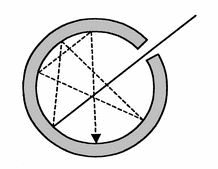
\includegraphics[scale=0.380]{16.png}}
\label{fig: cubed graph}
\end{figure}
\vspace*{-0.1}
Una volta realizzato il prototipo di un corpo nero, una volta assorbite le radiazioni elettromagnetiche, vediamo che tendenzialmente un corpo caldo emette onde elettromagnetiche piuttosto che assorbirne, poiché come si anticipava, in accordo con le affermazioni di Bolztmann, è più probabile che l'energia ed il calore passino da un corpo caldo ad uno freddo. Poiché sono entrambi corpi che emettono radiazioni, possiamo considerare il forno a microonde come esempio rudimentale di corpo nero.
\vspace*{-0.12in}
\paragraph{La distribuzione spettrale} Si osserva che lo spettro delle radiazioni emesse dal corpo nero non dipende dalle dimensioni del foro, né dalla composizione chimica delle pareti del corpo nero, che sono costanti,  ma dalla sua temperatura. L'irradianza $R$, o distribuzione spettrale dell'irradiamento, vale a dire l'energia emessa per unità volumica, è definita $R(\lambda, T)= \frac{P(\lambda, T)}{A\Delta \lambda} [\frac{W}{m^3}]$ come la potenza $[\frac{J}{S}]$ divisa per unità di superficie e lunghezza d'onda $[m^3]$. \\
Arrivando al punto nodale della questione: per l'elettromagnetismo classico, l'irradianza ha forma 
$R_1(\lambda, T) = \frac{8\pi}{c \lambda ^2} k_B T$ per la legge di Rayleigh-Jeans, dedotta dalle equazioni di Maxwell. 
\vspace*{-0.07in}
\paragraph{La catastrofe ultravioletta}
Questa funzione, graficata, produce enorme sgomento nella comunità scientifica. Sebbene riproduca gli andamenti attesi osservati in laboratorio a basse temperature, appena la temperatura si alza, per lunghezze d'onda appartenenti ai raggi ultravioletti, $R$ si avvicina ad infinito. Questa falla dell'elettromagnetismo classico sconvolse a tal punti i fisici da essere chiamata catastrofe ultravioletta.\\
\vspace*{-0.07}
Poiché l'integrale di questa curva, la sua area sottesa, ($R_1(\lambda, T) \times \lambda = E_R = \frac{\xi} {\Delta A} = $  ), è uguale all'irradiamento totale, l'asintoticità della curva è una palese violazione  del principio di conservazione dell'energia. Per lunghezze d'onda che tendono si avvicinano a 0,  la curva tende ad infinito. Per frequenze alte dunque, una radiazione elettromagnetica porterebbe irradiamento infinito. Il nostro microonde, arrivasse a temperature notevoli (sopra i $ 550K$), annichilirebbe il cibo.  Studiamo la funzione di Rayleigh-Jeans
\newpage
 \begin{figure}[h]
\centering
\frame{
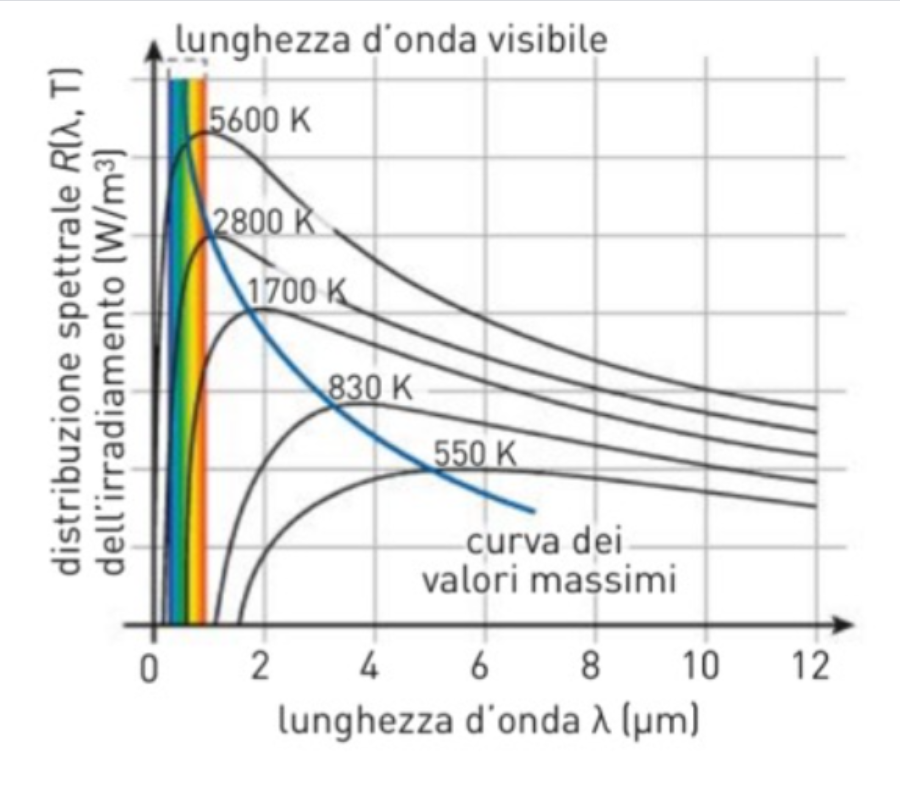
\includegraphics[scale=0.310]{28.png}}
\label{fig: cubed graph}
\end{figure}
Seguendo la curva dei massimi, per la quale per una lunghezza $\lambda_{max}$ corrisponde una $T_{max}$ secondo la legge di spostamento di Wien:
\[ T_{max} = \frac{2,90 \times 10^{-3} m\cdot K}{\lambda_{max} \]
vediamo che l'integrale di questa curva, l'irraggiamento, sarebbe infinito.
Prima di verificarlo matematicamente introduciamo il concetto di integrale definito.
\subsection{L'integrale definito}
\begin{quote}
    “The relationship between physics and mathematics goes back to the beginning of both
subjects; as the fields have advanced, this relationship has gotten more and more tangled, a
complicated tapestry. There is seemingly no end to the places where a well-placed set of
tools for making calculations could help physicists, or where a probing question from physics
could inspire mathematicians to create entirely new mathematical objects or theories.”
\end{quote}
L'integrale è una delle conferme storiche del legame profondo che vi è fra matematica e fisica, di come gli strumenti matematici aiutino la fisica e di come la fisica generi la necessità per della nuova matematica:teoremi strumenti e dimostrazioni. Pensando al novecento, le curvature di Riemann per la relatività o le matrici di Heisemberg per la meccanica quantistica, sono esempi lampanti di questa connessione. 
\\
Tornando all'integrale, questo nasce dalla necessità di calcolare aree di figure piane aventi un contorno curvilineo chiuso, che nel nostro caso ci aiuta a calcolare l'irradiamento generato da un corpo nero in funzione della lunghezza d'onda. 
\paragraph{Il metodo dei rettangoli} Possiamo vedere l'area sottesa di una curva come una somma $S$ di $n$ rettangoli che avranno base $\Delta x$. Se $n$ è veramente piccolo la somma che avremo sarà uguale all'area del trapezoide, l'area sottesa fra la curva e uno degli assi.
Data una funzione $f(x)$, continua in $[a;b]$, l'integrale definito all'interno dell'intervallo $[a;b]$ sarà il valore  limite per $\Delta x_{max}$ che tende a $0$ della somma dei rettangoli S.
\[ \int_a^b f(x)dx = \lim_{\Delta x_{max} \to 0 } \overline{S} =  \lim_{B\to 0}\sum_{i=1}^{n} B*h= \lim_{\Delta x\to 0}\sum_{i=1}^{n} \frac{b-a}{\Delta x}\cdot f(a+i \Delta x)\]
 \begin{figure}[h]
\centering
\frame{
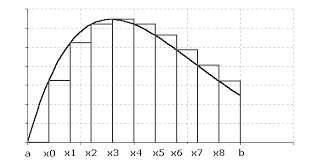
\includegraphics[scale=0.340]{29.png}}
\label{fig: cubed graph}
\end{figure}
\href{https://editor.p5js.org/freihm15@gmail.com/sketches/YjexPYqTc}{{\textit{\underline{Clicca qui per il metodo dei rettangoli in P5JS}}}}
\newpage
\subsection{Studio di Funzione: Irradianza di Rayleigh-Jeans}
\begin{center}
$R_1(\lambda, T) = \frac{8\pi}{c \lambda ^2} k_B T$ 
\end{center}
Per studiarla occorre una sostituzione di variabile $x = \lambda $.  Eliminiamo inoltre le costanti $k = \frac{8\pi}{c} k_B T$ poiché non rilevanti nello studio di funzione (Sono meramente coefficienti di dilatazione o contrazione). Troviamo: $R_1(x) = \frac{1}{x^2}$
\vspace*{-0.10in}
\paragraph{Tipo di funzione:} $R_1(x)$ é una funzione algebrica fratta.
\vspace*{-0.10in}
\paragraph{Dominio e segno:} $R_1(x) :\mathbb{R}^+ \to \mathbb{R}^+$ (costanti positive e $\lambda>0$, $R_1(x)>0 \ \forall x \in \textbf{D} $ )
\vspace*{-0.10in}
\paragraph{Intersezioni:} Non esistono intersezioni con gli assi. 
\vspace*{-0.10in}
\paragraph{Limiti:} Limiti agli estremi di definizione
\begin{itemize}
\item $\lim_{x \to \infty } \frac{1}{x^2} = 0^+ $\ \ \  y = 0 asintoto orizzontale dx 
\item $\lim_{x \to 0^+} \frac{1}{x^2}  = \infty $ \ \ \ x = 0 asintoto verticale dx $\to$ Violazione principio conservazione dell'energia
\end{itemize}
\\ La funzione è continua
\vspace*{-0.10in}
\paragraph{Derivate: massimi minimi e flessi:} Trovo le derivate prima e seconda e studio il segno
\begin{itemize}
    \item $R_1'(x) = \frac{-2}{x^3} \ \ \ R_1'(x)<0 \  \forall x \in \mathbb{R} \to$ funzione strettamente decrescente $\to$ non esistono massimi e minimi 
    \item $R_1''(x) = \frac{6}{x^4} \ \ \ R_1''(x)>0  \ \forall x \in \mathbb{R} \to$ funzione a concavità positiva $\to$ non esistono punti di flesso
\end{itemize}

\vspace*{-0.20in}

 \begin{figure}[h]
\centering
\frame{
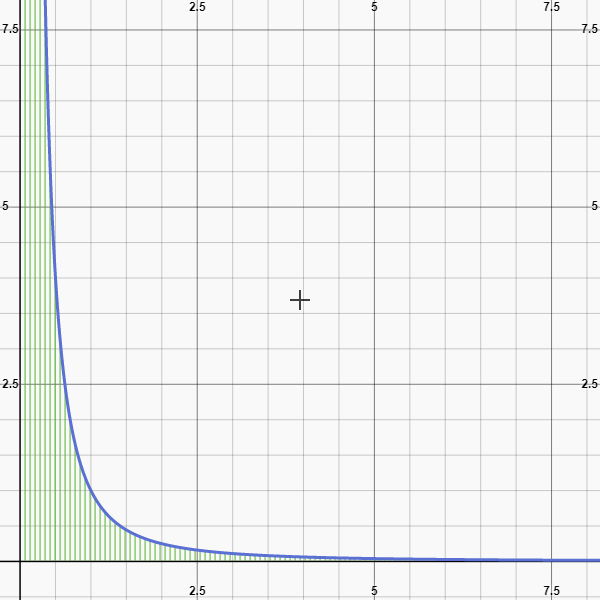
\includegraphics[scale=0.1800]{18.png}}
\label{fig: cubed graph}
\end{figure}
\vspace*{-0.20in}
\paragraph{Integrazione:} Svolgiamo integrale improprio della funzione per dimostrare l'inconsistenza della legge con il principio conservazione dell'energia.\\ Applichiamo l'integrale indefinito. Prendendo il punto $P(1;1) \in R(x)$ come riferimento
\begin{center}
\vspace*{-0.10in}
\[ \int_{0^+}^{+\infty} R_1(x)dx  
= \lim_{t\to 0^+} \int_{t}^{1}R_1(x)dx  + \lim_{z\to +\infty} \int_{1}^{z}R_1(x)dx \ \ \ 
\\ \text{con}\  t = 0 \wedge \ z = +\infty \]
\end{center}
Trovo la primitiva di $R_1(x)$  che chiamiamo $R_1^*(x)$:\ \  $R_1^*(x) = -\frac{1}{x} + C $
\\ Svolgiamo entrambi i limiti degli integrali 
\begin{enumerate}
\item \[ \lim_{t\to 0^+} \int_{t}^{1}R_1(x)dx\ = \lim_{t \to 0^+} \left[ -\frac{1}{x^2} \right]_t^1 = \lim_{t \to 0^+} -1 +\frac{1}{t^2} = +\infty \]
\item \[ \lim_{z\to +\infty} \int_{1}^{z}R_1(x)dx \ \ \lim_{z \to +\infty } \left[ -\frac{1}{x^2} \right]_1^z = \lim_{z \to \infty} 0 - \left( -\frac{1}{t^2} \right) = 1 \]
\end{enumerate}
L'integrale numero 1 è uguale a $+\infty$ ed è dunque divergente: la regione integrata non è limitata ed ha una area infinita
L'integrale numero 2 è uguale a $1$ ed è dunque convergente: la regione integrata non è limitata ma ha un'area finita.
Poiché l'integrale di una somma è uguale alla somma degli integrali degli addendi, l'integrale totale è divergente: il principio della conservazione dell'energia non è rispettato.   
\newpage
\subsection{I quanti di Planck}
\paragraph{Pacchetti energetici}
Le misure sperimentali, naturalmente, non pongono alcun problema dal punto di vista della conservazione dell'energia.
Max Planck nel 1900, risolve, a suo dire attraverso un artificio matematico, la catastrofe ultravioletta.  Affinché la distribuzione spettrale dell'irradiamento non sia infinita per lunghezze d'onda incirca uguali agli ultravioletti, è necessario che gli scambi energetici fra atomi, molecole all'interno della cavità del corpo nero e dunque all'interno del nostro microonde, avvengano attraverso il passaggio di pacchetti di energia. Da un passaggio continuo di energia, che portava l'irradianza ad infinito, si passa allo scambio di pacchetti energetici, definiti quanti del campo elettromagnetico o semplicemente quanti.
 \begin{figure}[h]
\centering

\includegraphics[scale=0.340]{21.png} $\to$

\includegraphics[scale=0.340]{20.png}
\label{fig: cubed graph}
\end{figure}\\
Secondo Planck, l'energia scambiata dalle onde elettromagnetiche assumerebbe esclusivamente valori discreti, da cui la $n \in \mathbb{N}$, e
sarebbe direttamente proporzionale alla frequenza delle onde elettromagnetiche.
\begin{center}
    $E = nhf$
\end{center}
$h$ è detta costante di Planck. $h = 6,62607 \times 10^{-34} J \cdot s$. È una costante di ordine così basso che la quantizzazione non è percettibile e uno scambio di energia continuo appare ragionevole per frequenze di uso ordinario. Il prodotto tra $h$ ed $f$
Questa soluzione provocò molto disorientamento nella comunità scientifica, tant'è che lo stesso Planck era scettico nel considerarla legittima ma le conferme sperimentali non tardarono ad arrivare.
\paragraph{L'irradianza di Planck}
Planck, concependo lo scambio pacchettizzato, discreto, di energia, riesce a dare una nuova forma all'Irradianza R: 

\begin{center}
    $ R_2(\lambda, T) = \frac{2\pi c^2}{\lambda^5} \frac{h}{e^{\frac{hc}{\lambda k_B T} }-1} $
\end{center}
Questa funzione, graficata, riproduce gli  andamenti sperimentali. Confrontiamola con l'Irradianza di Planck. 
\begin{figure}[h]
\centering
\frame{
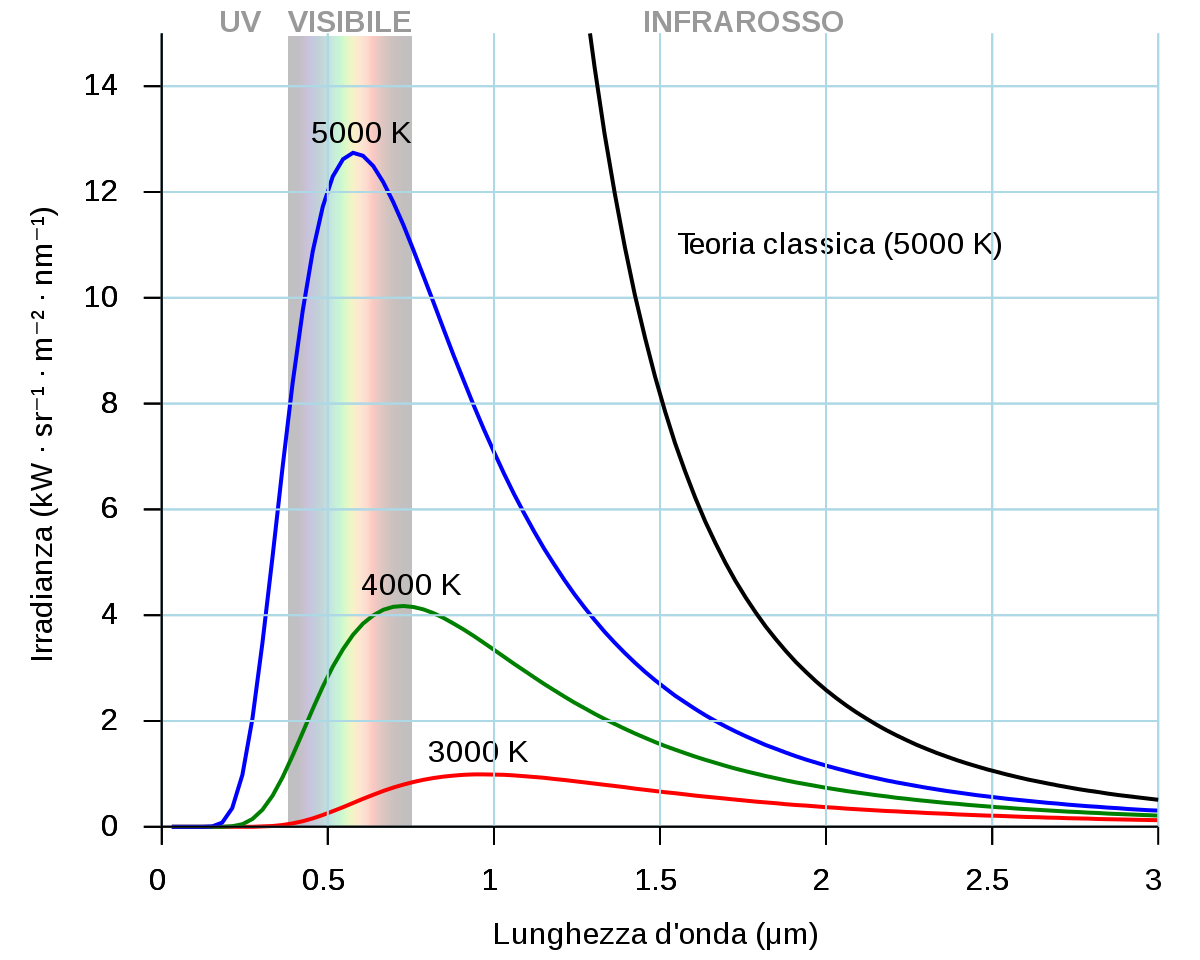
\includegraphics[scale=0.1400]{17.png}}
\end{figure}
\\
L'integrale di questa curva, equivalente alla sua area sottesa e dunque al suo irradiamento, al variare della temperatura, è limitato,  sarà dunque in accordo con il principio di conservazione dell'energia.
Studiamo la funzione:
\newpage
\subsection{Studio di funzione: Irradianza di Planck}
\begin{center}
     $ R_2(\lambda, T) = \frac{2\pi c^2}{\lambda^5} \frac{h}{e^{\frac{hc}{\lambda k_B T} }-1} $

\end{center}
Per studiare la funzione sostituiamo: $x = \lambda$ nell'equazione sopra riportata ed eliminiamo tutti i parametri costanti che concorrono solo alla dilatazione o alla contrazione della funzione. Studiamo
\begin{center}
    $R_2(x) = \frac{1}{x^5 \ (e^{\frac{1}{x } }-1)}$
\end{center}
\vspace*{-0.20in}
\paragraph{Tipo di funzione:} $R_2(x)$ é una funzione trascendente fratta.
\vspace*{-0.10in}
\paragraph{Dominio e segno:} $R_2(x) :\mathbb{R}^+ \to \mathbb{R}^+$ (costanti positive e $\lambda>0$, $R_1(x)>0 \ \forall x \in \textbf{D} $ )
\vspace*{-0.10in}
\paragraph{Intersezioni:} Non esistono intersezioni con gli assi. 
\vspace*{-0.10in}
\paragraph{Limiti:} Limiti agli estremi di definizione
\begin{itemize}
\item  $\lim_{x \to \infty } \frac{1}{x^5 \ (e^{\frac{1}{x } }-1)}  = \frac{1}{\infty \cdot 0} = 0 \cdot \infty \ F.I. $ passo a De L'Hospital$ \\ 
$\lim_{x \to \infty } \frac{1}{x^5 \ (e^{\frac{1}{x } }-1)} = \lim_{x \to \infty } \frac{ D[x^{-5}]}{D[e^\frac{1}{x}-1]} = \lim_{x \to \infty } - \frac{5}{x^{6} \cdot (-)e^\frac{1}{x} \frac{1}{x^2}} = \lim_{x \to \infty }  \frac{5}{x^{4} \cdot e^\frac{1}{x}} = 0^+ \\ $ y = 0 asintoto orizzontale dx 
\item $ \lim_{x \to 0} \frac{1}{x^5 \ (e^{\frac{1}{x } }-1)}  = \frac{1}{0 \cdot \infty}  = \infty \cdot 0 \ F.I.$ passo a De L'Hospital \\
$ \lim_{x \to 0 } \frac{1}{x^5 \ (e^{\frac{1}{x } }-1)} = \lim_{x \to 0 } \frac{ D[x^{-5}]}{D[e^\frac{1}{x}-1]} = \lim_{x \to 0 } - \frac{5}{x^{6} \cdot (-)e^\frac{1}{x} \frac{1}{x^2}} = \lim_{x \to 0 }  \frac{5}{x^{4} \cdot e^\frac{1}{x}} = \frac{5}{0 \cdot \infty} =  \infty \cdot 0 \ F.I.$ \\ Riapplico de L'Hospital \\
$\lim_{x \to 0 }  \frac{5}{x^{4} \cdot e^\frac{1}{x}} \to $ 3 volte de L'Hospital $ \to \lim_{x \to 0} \frac{120}{e^\frac{1}{x}} = 0^+$

\end{itemize}
\vspace*{-0.10in}
\paragraph{Derivata prima:} Massimi e minimi \\
$R_2'(x) = -\frac{\left(5x-1\right)\mathrm{e}^\frac{1}{x}-5x}{x^7\left(\mathrm{e}^\frac{1}{x}-1\right)^2}$ 
Studiamo:
\begin{enumerate}
    \item N1: $e^{1/x}>\frac{5x}{5x -1}$ che studiamo con un confronto grafico $e^{1/x}=\frac{5x}{5x -1}$ in $x_M$  $e^{1/x}>\frac{5x}{5x -1}>0 $ per $x>x_M$ 
    \item D1: $-x^7>0$ per $x<0$
    \item D2: $(e^{1/x}-1)>0 \forall x \in \mathbb{R}$
\end{enumerate}
Facciamo il grafico dei segni:\\
\vspace*{-0.2in}
\begin{figure}[h]
\centering
\frame{
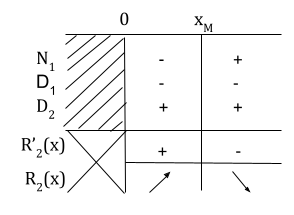
\includegraphics[scale=0.300]{27.png}}
\end{figure}
\vspace*{-1.1in}
Avremo
\begin{enumerate}[noitemsep]
    \item $R_2'(x)>0$ per $0<x<x_M$
    \item $R_2'(x)=0$ per $x=x_M$
    \item $R_2'(x)<0$ per $x>x_M$ 
\end{enumerate}
La derivata sarà dunque: 

\end{enumerate}
\begin{figure}[h]
\centering
\frame{
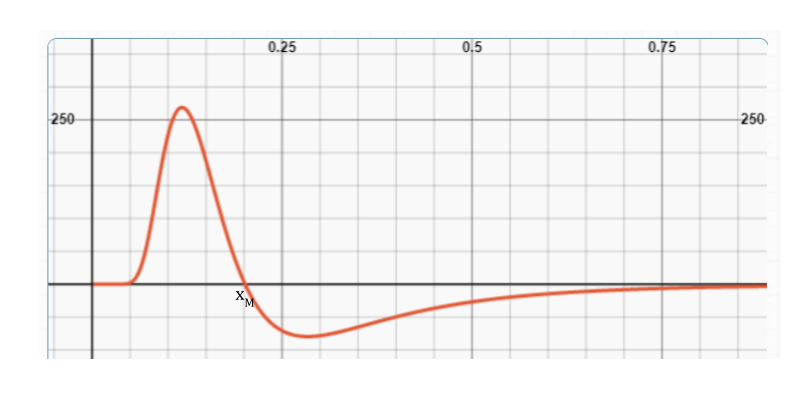
\includegraphics[scale=0.2800]{26.png}}
\end{figure}
\newpage
\paragraph{ Grafico:} Grafichiamo la funzione
\\

\begin{figure}[h]
\centering
\frame{
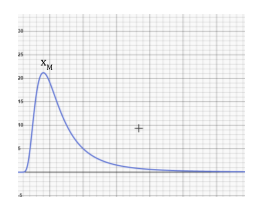
\includegraphics[scale=0.530]{23.png}}
\end{figure}

\vspace*{-0.10in}
\paragraph{Integrazione:} Svolgiamo l'integrale della funzione irradianza di Planck \\
Portiamo fuori le costanti. 
\[ \int_0^\infty R(\lambda )d\lambda = 2\pi c^2h \int_0^\infty \frac{1}{\lambda^5(e^\frac{hc}{k_B\lambda T})-1}\] 
Per risolvere l'integrale conviene operare un cambiamento di variabile 
\[ x = \frac{hc}{kT\lamba} \to \lambda = \frac{hc}{kTx} \]
Inoltre per la definizione di differenziale:
\[ d \lambda = f'(x) \cdot dx  = - \frac{hc}{kT \ x^2} dx\]
Detto questo possiamo scrivere l'integrale come 
\[ \int_0^\infty 2\pi \frac{k_B^4 T^4}{h^3 c^2} \int_0^\infty \frac{x^3}{e^x-1}dx\]
Si può dimostrare che
\[ \int_0^\infty \frac{x^3}{e^x-1}dx = \frac {3 \pi^4}{15}\]

\paragraph{Dimostrazione dell'integrale: }
In generale vale che: 
\[[1]: \ \  I_n = \int_0^\infty \frac{x^n}{e^x-1}dx = \int_0^\infty x^n\sum_{i=1}^{\infty} e^{-ix}dx \]
La sommatoria introdotta è una serie geometrica caratterizzata dall'andamento
\[\sum_{n=0}^{\infty}q^n = 1 + q + q^2 + q^3 + ... + q^n + ...\]\\
Se consideriamo la serie geometrica $e^{-ix}$, poiché $n = -ix$ è considerata una serie parte delle serie che hanno $q<1$ perché:\\
\begin{cent}
se $x>0$ allora l'esponenziale $e^{-x} \in (0,1) \to 0<e^{-x}<1$
\end{cent}
\\Le serie geometriche di ragione $q<1$ si risolvono: 
\[ \sum_{n=0}^{\infty} q^n = \frac{1}{1-q}\]
Applicando questa proprietà abbiamo
\[ \sum_{n=0}^{\infty} e^{-x} = \frac{1}{1-e^{-x}} = \frac{1}{1-\frac{1}{e^x}} = \frac{e^x}{e^x-1}\]
E dunque
\[ [2]: \ \ \sum_{n=1}^{\infty} e^{-x} = \sum_{n=0}^{\infty} e^{-x} -1  = \frac{e^x}{e^x-1} -1 =  \frac{e^x-e^x + 1}{e^x -1} = \frac{1}{e^x -1} \]
Una volta dimostrato la [2], vale la [1]. Poiché l'integrale di una somma è la somma degli integrali vale dunque 
\[ I_n = \sum_{i=1}^{\infty} \int_0^\infty x^n e^{-ix}dx \]
Se sostituiamo $t = ix$ avremo
\[ I_n = \sum_{i=1}^{\infty} \frac{1}{i^{n+1}} \int_0^\infty t^n e^{-t}dt \]  
L'integrale $\int_0^\infty t^n e^{-t}dt $ uguale alla funzione Gamma $\Gamma (n+1)$ di Eulero che per argomenti naturali è $n!$
\[\int_0^\infty t^n e^{-t}dt = \Gamma (n+1) = n!\]  
Possiamo scrivere che 
\[ I_n = n! \sum_{i=1}^{\infty} \frac{1}{i^{n+1}}\]  
Introduciamo la funzione zeta $\zeta$ di Riemann $\zeta (n)=\sum_{i=1}^{\infty} \frac{1}{i^{n}} = 1 + \frac{1}{2^n} + \frac{1}{3^n}+ \frac{1}{4^n}}$ 
Otteniamo infine che 
\[ I_n = n! \zeta(n+1)\]  
Valori della funzione $\zeta$ sono stati calcolati da Eulero ed abbiamo che: $n = 3   \to I_n = 3\frac{\pi^4}{15} $
\\L'integrale è dunque definito: La regione integrata non è limitata ma ha un'area finita.
\begin{figure}[h]
\centering
\frame{
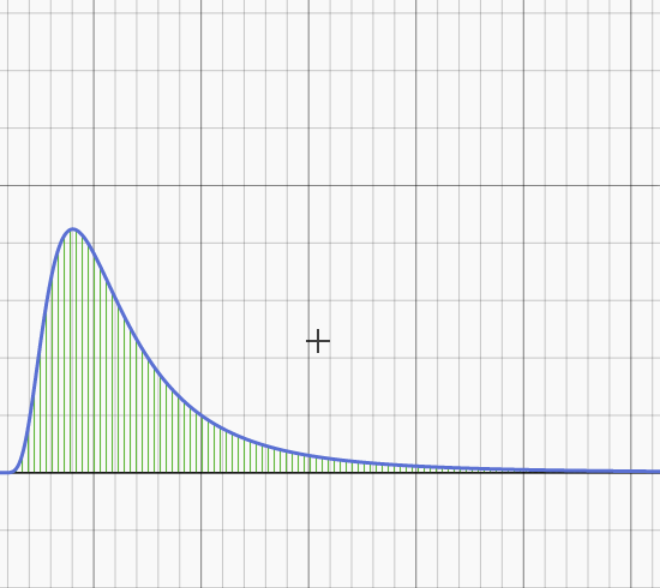
\includegraphics[scale=0.4000]{22.png}}
\end{figure}
\newpage
\subsection {Prove empiriche della quantizzazione della luce}
\paragraph{Fireworks!} Potremmo provare il comportamento quantizzato e quindi corpuscolare della luce mettendo un cucchiaio all'interno della cavità di cottura.
L'acciaio inox, una lega di ferro, irradiato dalle onde elettromagnetiche, potrebbe emettere elettroni per effetto fotoelettrico. 
\begin{figure}[h]
\centering
\frame{
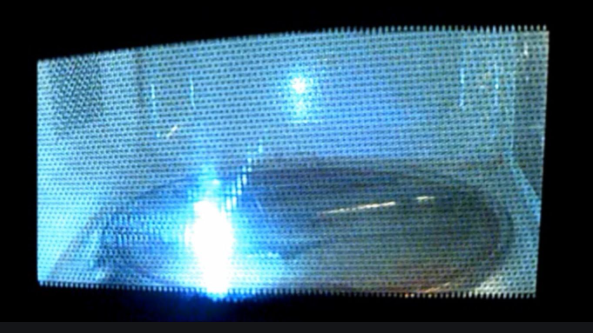
\includegraphics[scale=0.3000]{24.png}}
\end{figure}\\
L'emissione di elettroni da parte da un materiale ferromagnetico è una delle prove empiriche del comportamento quantizzato e quindi corpuscolare della luce.
Einstein nel 1905 sposa la teoria di Planck: la radiazione elettromagnetica è composta da singoli pacchetti di energia: i fotoni.
I fotoni hanno energia: 
\[ E = hf\]
Possiamo ricavare dall'espressione della quantità di moto relativistica del quadrivettore energia quantità di moto:
\[ \left( \frac{E}{c} \right)^2 + P^2 = m_0^2c^2 \to P = \sqrt{\left( \frac{E}{c} \right)^2 - m_0^2c^2}  = \frac{E}{c} = \frac{hf}{c}\]
In realtà, poiché la soglia fotoelettrica (la frequenza da superare affinché avvenga l'emissione di elettroni) dell'acciaio inox è maggiore della frequenza delle microonde non si tratta di effetto fotoelettrico.
\[ f_{min}> f_{microonde} \to \frac{W_{estrazione}}{h} >\frac{c}{\lambda_{microonde}}\]
 Assumendo che le microonde fossero state onde elettromagnetiche di frequenza maggiore avremmo assistito all'emissione di elettroni, la cui energia era stata rimpiazzata con l'assorbimento dell'energia del fotone da parte del catodo, il cucchiaio,  in seguito ad  un urto completamente elastico, che conserva energia e quantità di moto.
\paragraph{Zap!} Nel nostro caso, l'apparizione di scintille, di una corrente e dunque di elettroni, non è sintomo dell'effetto fotoelettrico e quindi dell'emissione di elettroni spontanea dovuta all'irraggiamento delle onde elettromagnetiche.
\\

Il cucchiaio, realizzato in materiale ad alta conduzione, possiede una curvatura che crea acute differenze di potenziale all'interno della sua superficie. Gli elettroni liberi al suo interno non si distribuiscono in modo uniforme creando un forte campo elettrico che va a ionizzare le molecole ed i gas nell'aria che permettono, una volta rotta la rigidità dielettrica, il passaggio di corrente fra due polarità opposte e dunque della scintilla.
La creazione di scintille è determinata quindi non dalle onde elettromagnetiche ma dalla disomogeneità della superficie irradiata. Una sfera all'interno di un microonde non produrrebbe scintille.
\subsection{Chiudere il cerchio} 
Per chiudere il cerchio, possiamo osservare che la luce si presenti come onda o come flusso di particelle a seconda delle condizioni sperimentali. Einstein con l'effetto fotoelettrico, Bohr con il suo modello atomico, e Planck con la distribuzione spettrale dell'irradiamento all'interno del corpo nero, dimostrano tutti che la fisica classica ed il modello ondulatorio della luce non erano in grado di descrivere i fenomeni microscopici. 
\paragraph{La rivoluzionarietà dell'elettromagnetismo} La rivoluzionarietà dell'elettromagnetismo di Faraday e Maxwell, sta dunque nel far emergere questa contraddizione che porta allo nascita della meccanica quantistica. L'elettromagnetismo come antitesi alla fisica classica.
\paragraph{La dualità onda-particella della luce} Il comportamento duplice della luce è messo in luce dalla lunghezza d'Onda di De Broglie:
\[ \lambda = \frac{h}{p}\]
con $p$ quantità di moto del fotone e $\lambda$ lunghezza d'onda dell'onda elettromagnetica.\\

Alla scoperta che sia le radiazioni elettromagnetiche, sia le particelle materiali mostrano in alcuni fenomeni una natura ondulatoria ed in altri corpuscolari, entra in gioco Heisemberg, letteralmente la fine dei giochi.\\

Il suo principio di indeterminazione ci svela che, come per osservare un oggetto bisogna illuminarlo, osservando un elettrone e quindi osservando il comportamento di una particella o di un'onda la illuminiamo. Misurando ad esempio la sua posizione, andremo a modificare imprevedibilmente la sua quantità di moto irradiandola con altri fotoni. Il principio di indeterminazione ci occlude così il mondo microscopico, che rimane per noi, citando Schopenhauer, rappresentazione.
\newpage
\section{Bibliografia e Sitografia}
\subsection{Bibliografia}
\begin{itemize}[noitemsep]
    \item ``La realtà non è come ci appare. La struttura elementare delle cose" ‒ Carlo Rovelli 
    \item ``Sette brevi lezioni di fisica" ‒ Carlo Rovelli
    \item ``Helgoland" ‒ Carlo Rovelli
    \item ``Matematica.blu 2.0" - Massimo Bergamini, Graziella Barozzi, Anna Trifone
    \item ``L'amaldi per i licei scientifici.blu Onde, Campo Elettrico e Magnetico" - Ugo Amaldi
    \item ``L'amaldi per i licei scientifici.blu Induzione e Onde elettromagnetiche, Relatività e Quanti" - Ugo Amaldi
\end{itemize}
\subsection{Sitografia}
\begin{itemize}[noitemsep]
    \item Il forno a microonde 
    \begin{itemize}[noitemsep]{
    \item \url{https://iopscience.iop.org/article/10.1088/0031-9120/39/1/006}
     \item\url{https://it.wikipedia.org/wiki/Forno_a_microonde}
    \end{itemize}
    \item Raddrizzatore 
\begin{itemize}[noitemsep]
\item \url{https://it.wikipedia.org/wiki/Raddrizzatore}
\end{itemize}
    \item Funzionamento del magnetron  
\begin{itemize}[noitemsep]
\item \url{https://www.radartutorial.eu/08.transmitters/Magnetron.en.html}
\end{itemize}
    \item Riscaldamento a Microonde 
\begin{itemize}[noitemsep]
\item \url{https://www.comsol.com/multiphysics/microwave-heating?parent=electromagnetics-072-122}
\end{itemize}
    \item Catastrofe ultravioletta 
\begin{itemize}[noitemsep]
\item \url{http://www.robertobigoni.it/Fisica/Planck/Planck.html}
\item \url{https://fsigward.files.wordpress.com/2013/09/lezione-07-corpo-nero-e-ipotesi-di-planck.pdf}
\end{itemize}
\end{itemize}
\subsection{Multimedia}
\begin{itemize}[noitemsep]
  \item Funzionamento del microonde:
  \begin{itemize}[noitemsep]
   \item \url{https://www.youtube.com/watch?v=kp33ZprO0Ck}
   \item \url{https://www.youtube.com/watch?v=lVu11WWrNbQ} 
  \end{itemize}
  \item Funzionamento del magnetron
\begin{itemize}[noitemsep]
\item \url{https://www.youtube.com/watch?v=bUsS5KUMLvw}
\end{itemize}
  \item Catastrofe ultravioletta 
  
\begin{itemize}[noitemsep]
\item \url{https://www.youtube.com/watch?v=7BXvc9W97iU}
\end{itemize}
\end{itemize}
\begin{quote}

\end{quote}


\end{document}
